% \chapter{N-Fold via LP rounding} \label{platform}
\newpage
\section{N-Fold via LP rounding}  % Set the left side page header

The main drawback for improving the complexity of the augmentation algorithm is that after solving the linear relaxation, we can be arbitrarily far from the optimal solution of the IP, what means that we need many augmentation steps. In this section we follow another approach introduced in \cite{EISENBRAND:2020} based on a more restricted linear relaxation which optimum is closer to the optimum of the IP and we prove this. We then show how to take advantage of this proximity bound to obtain the current fastest algorithm for the N-Fold case, running in roughly linear time.


\subsection{Restricted linear relaxation}
% TODO: Not going deeper but references or really short explanation
\begin{proposition}[\textbf{N-Fold RLR complexity}]
    The N-Fold IP restricted linear relaxation problem can be solved in time
    \begin{equation*}
        O(nt \cdot log^2(nt) \cdot \varphi p(r) (s\Delta)^{O(s^2)})
    \end{equation*}
\end{proposition}

\begin{figure}[h]
\centering
\begin{minipage}[b]{0.45\textwidth}
    \centering
    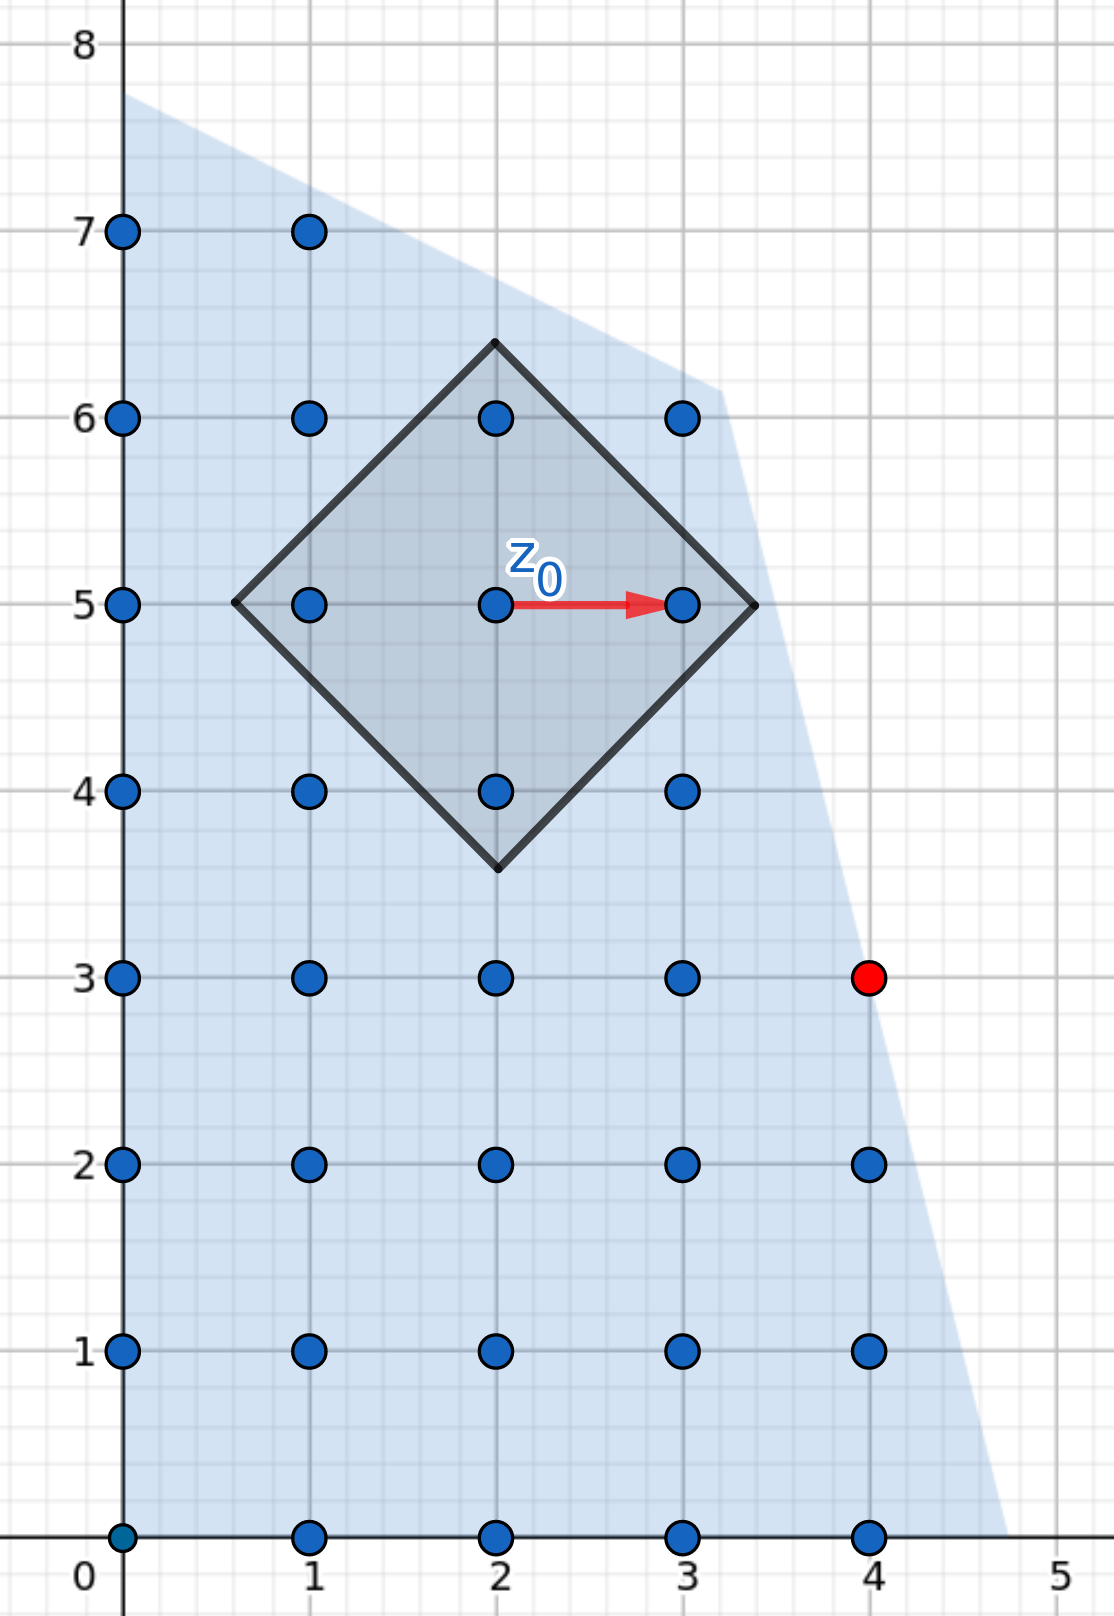
\includegraphics[width=0.9\textwidth]{images/IP(6).png}
    % TODO!
    \caption{Complete this}
\end{minipage}
\hfill
\begin{minipage}[b]{0.45\textwidth}
    \centering
    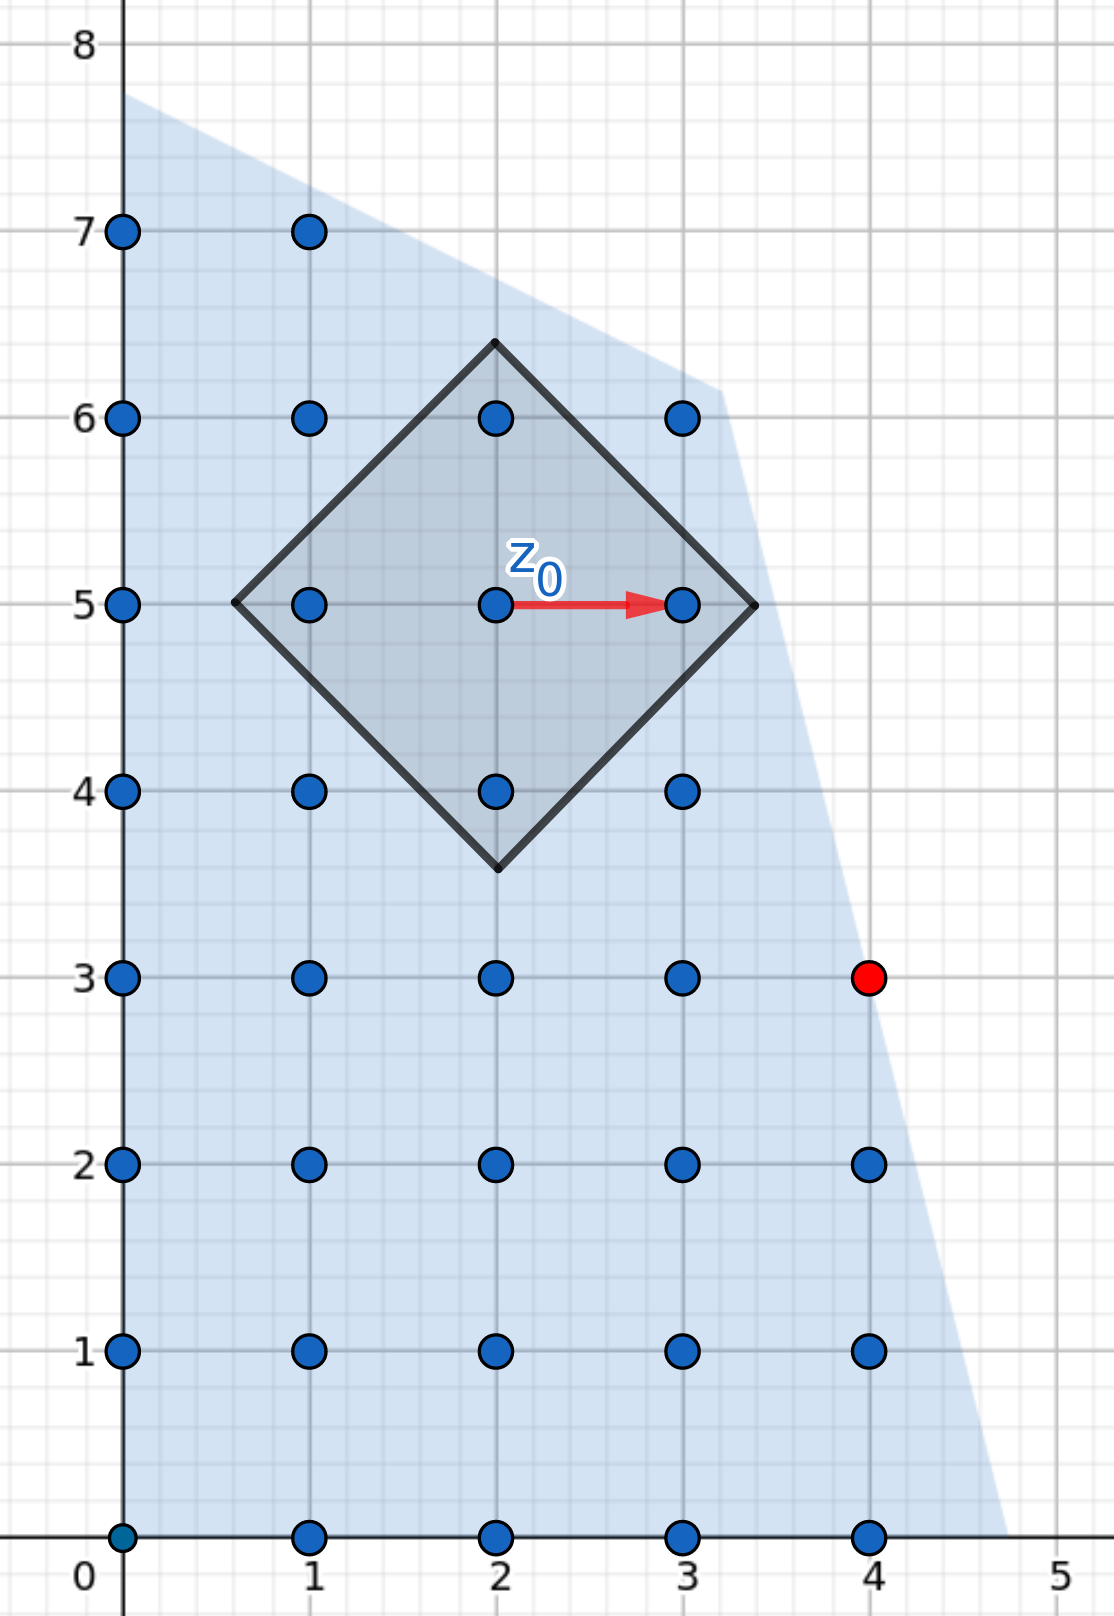
\includegraphics[width=0.9\textwidth]{images/IP(6).png}
    % TODO!
    \caption{Also this}
\end{minipage}
\end{figure}

\newpage
\subsection{Dynamic program}        
% TODO: Proof? At least explanation or references
\begin{proposition}[\textbf{N-Fold RLR to optimum complexity}]
    Given an optimal vertex of an N-Fold RLR, the N-Fold IP can be solved in time
    \begin{equation*}
        O(nt \cdot (rs\Delta)^{O(r^2s+s^2)})
    \end{equation*}
\end{proposition}
%\hspace{15pt}[Cslovjecsek, Eisenbrand, Weismantel 2020]

\begin{proposition}[\textbf{N-Fold proximity to RLR}]
    Let $x^*$ be an optimal vertex solution of a N-Fold RLR, then there exists an optimal solution $z^*$ for the N-Fold IP verifying:  
    \begin{equation*}
        ||z^* - x^*||_1 \leq (rs\Delta)^{O(rs)}
    \end{equation*}
\end{proposition}
\hspace{15pt}[Cslovjecsek, Eisenbrand, Weismantel 2020]



Graph plot for the proof of algorithm complexity:
------------------------------------------------------
\begin{center}
\begin{tikzpicture}[
        > = stealth, % arrow head style
        shorten > = 1pt, % don't touch arrow head to node
        auto,
        node distance = 3cm, % distance between nodes
        semithick % line style
    ]

    \tikzstyle{every state}=[
        draw = black,
        thick,
        fill = white,
        minimum size = 4mm
    ]

    \node[state, minimum size=0.8cm] (s) at (0,0) {$0$};
    
    %\node[state] (w1) at (2,2)  {$y_{11}$};
    %\node[state] (u1) at (2,0)  {$y_{12}$};
    \node[state] (v1) at (2,-2) {$y_{13}$};
    
    %\node (u2) at (4,0)  {$\sum_{i=1}^\ell A_ix^*$};
    \node[state] (w2) at (4,2)  {$y_{21}$};
    %\node[state] (u2) at (4,0)  {$y_{22}$};
    %\node[state] (v2) at (4,-2) {$y_{23}$};
    
    %\node[state] (w3) at (6,2)  {$y_{31}$};
    \node[state] (u3) at (6,0)  {$y_{32}$};
    %\node[state] (v3) at (6,-2) {$y_{33}$};
    
    \node[state] (w4) at (8,2)  {$y_{41}$};
    %\node[state] (u4) at (8,0)  {$y_{42}$};
    %\node[state] (v4) at (8,-2) {$y_{43}$};
    
    \node[state, minimum size=0.8cm] (f) at (10,0)  {$b_0$};
    
    \path[->] (s) edge node  {$c_1^tu_1^*$} (v1);
    \path[->] (v1) edge node {$c_2^tu_2^*$} (w2);
    \path[->] (w2) edge node {$c_3^tu_3^*$} (u3);
    \path[->] (u3) edge node {$c_4^tu_4^*$} (w4);
    \path[->] (w4) edge node {$c_5^tu_5^*$} (f);

    \draw[red, dashed] (1, 3) -- (1, -3);
    \draw[red, dashed] (3, 3) -- (3, -3);
    \draw[red, dashed] (5, 3) -- (5, -3);
    \draw[red, dashed] (7, 3) -- (7, -3);
    \draw[red, dashed] (9, 3) -- (9, -3);
    
    % \node (S1) at (2,-3.5) {$S_1$};
    % \node (S2) at (4,-3.5) {$S_2$};
    % \node (S3) at (6,-3.5) {$S_3$};
    % \node (S4) at (8,-3.5) {$S_4$};
\end{tikzpicture}
\end{center}

Graph plot for the proof of algorithm complexity:
------------------------------------------------------

\begin{center}
\begin{tikzpicture}[
        > = stealth, % arrow head style
        shorten > = 1pt, % don't touch arrow head to node
        auto,
        node distance = 3cm, % distance between nodes
        semithick % line style
    ]

    \tikzstyle{every state}=[
        draw = black,
        thick,
        fill = white,
        minimum size = 4mm
    ]

    \node[state, minimum size=0.8cm] (s) at (0,0) {$0$};
    
    %\node[state] (w1) at (2,2)  {$y_{11}$};
    %\node[state] (u1) at (2,0)  {$y_{12}$};
    \node[state] (v1) at (2,-2) {$y_{13}$};
    
    %\node (u2) at (4,0)  {$\sum_{i=1}^\ell A_ix^*$};
    \node[state] (w2) at (4,2)  {$y_{21}$};
    %\node[state] (u2) at (4,0)  {$y_{22}$};
    %\node[state] (v2) at (4,-2) {$y_{23}$};
    
    %\node[state] (w3) at (6,2)  {$y_{31}$};
    \node[state] (u3) at (6,0)  {$y_{32}$};
    %\node[state] (v3) at (6,-2) {$y_{33}$};
    
    \node[state] (w4) at (8,2)  {$y_{41}$};
    %\node[state] (u4) at (8,0)  {$y_{42}$};
    %\node[state] (v4) at (8,-2) {$y_{43}$};
    
    \node[state, minimum size=0.8cm] (f) at (10,0)  {$b_0$};
    
    \path[->] (s) edge node  {$c_1^tu_1^*$} (v1);
    \path[->] (v1) edge node {$c_2^tu_2^*$} (w2);
    \path[->] (w2) edge node {$c_3^tu_3^*$} (u3);
    \path[->] (u3) edge node {$c_4^tu_4^*$} (w4);
    \path[->] (w4) edge node {$c_5^tu_5^*$} (f);

    \draw[red, dashed] (1, 3) -- (1, -3);
    \draw[red, dashed] (3, 3) -- (3, -3);
    \draw[red, dashed] (5, 3) -- (5, -3);
    \draw[red, dashed] (7, 3) -- (7, -3);
    \draw[red, dashed] (9, 3) -- (9, -3);
    
    % \node (S1) at (2,-3.5) {$S_1$};
    % \node (S2) at (4,-3.5) {$S_2$};
    % \node (S3) at (6,-3.5) {$S_3$};
    % \node (S4) at (8,-3.5) {$S_4$};
\end{tikzpicture}
\end{center}

\textbf{Facts for N-Fold complexity}
\begin{itemize}
    \item $|S_l| \leq (rs\Delta)^{O(r^2s)}$
    \item $|V| + |E| \leq O(n(rs\Delta)^{O(r^2s)})$
    \item The edge IP can be computed in time $t((r + s)\Delta)^{O(r + s)^2}$
    \item Longest path problem in a acyclic digraph can be solved in linear time.
\end{itemize}

\textbf{N-Fold complexity}
\begin{itemize}
\item \textbf{N-Fold complexity}\\
    The N-Fold IP can be solved in time $nt(rs\Delta)^{O(r^2s + s^2)} + RLR$
\end{itemize}
\hspace{15pt}[Cslovjecsek, Eisenbrand, Weismantel 2020]